\chapter{Evaluación del cumplimiento de las reglas sobre el caso de estudio}
\label{capitulo6}

\section{Introducción}
\label{capitulo6:introduccion}

\emph{Diaspora} es una aplicación que se utiliza todos los días por miles de usuarios que comparten contenido. Por su naturaleza de código abierto, se modifica
constantemente, muchas veces por individuos que no tienen un conocimiento avanzando de \emph{Ruby on Rails} ni de buenas prácticas en el desarrollo web. Sin embargo, todas las
modificaciones realizadas deben ser validadas por un comité de pocas personas que tienen privilegios de modificación al repositorio. Las personas que tienen estos privilegios son los
creadores de la aplicación, y otras personas que entraron por méritos generados a través de aportes para la misma. Desde hace un tiempo \emph{Diaspora} es un proyecto de la 
comunidad, esto quiere decir que la comunidad es la encargada de determinar el rumbo del futuro de la aplicación y de mantenerla. No existe ningún desarrollador cuyo trabajo sea 
mantener \emph{Diaspora}, todo el mantenimiento se realiza por la voluntad de los desarrolladores. Esto tiene algunas consecuencias como por ejemplo que el calendario de 
liberaciones sea un tanto errático ya que no hay un ciclo formal de desarrollo establecido. 

Muchas de las personas que aportan código a \emph{Diaspora} no son desarrolladores web, y realizan aportes por el simple interés de mejorar la aplicación.
Muchas veces, cuando los contribuidores proponen modificaciones al código, no prestan atención a detalles de su solución que dañan a la performance de la aplicación debido a la
falta de conocimiento sobre las buenas prácticas. Al incorporar un cambio, simplemente se verifica que las modificaciones tengan pruebas funcionales, y no produzcan regresiones en 
viejas funcionalidades. Como se ha visto, la performance es un requerimiento no funcional, difícil de probar e incorporar en el desarrollo para personas que no se dedican al 
desarrollo web como profesión. Como consecuencia, el código de \emph{Diaspora} no cumple con algunas de las reglas vistas en la sección \ref{capitulo3:reglas}, y 
tampoco, en muchos casos con las convenciones y patrones típicos de aplicaciones \emph{Ruby on Rails}. En este Capítulo se detallan los problemas encontrados al analizar el 
código de \emph{Diaspora} junto a su resolución.

\section{Metodología de trabajo}

Para cada una de las reglas presentadas en la sección \ref{capitulo3:reglas} se analizó el cumplimiento de las mismas por parte de la aplicación utilizando las herramientas 
\emph{Page Speed} e \emph{YSlow}. Este análisis reveló que \emph{Diaspora} se encontraba en falta con algunas reglas presentadas, lo cual daba lugar a posibles espacios de 
mejora de performance.

A continuación se presenta para cada una de las reglas no cumplidas, cuales son las implementaciones realizadas por el equipo para mejorar la performance de la aplicación.
Además del incumplimiento de las reglas, el código fue analizado en busca de mejoras de otros tipos, entre ellas, detección de código muerto innecesario, y problemas de consultas
en bases de datos los cuales también fueron solucionados por el equipo.

Algunas mejoras fueron implementadas completamente y otras parcialmente debido al estado del código. En algunos casos, la reestructura necesaria en el código actual para
implementar una mejora era demasiado alta y se cree que escapa del alcance de este proyecto. De todas maneras, es posible llevar a cabo estas reestructuras como trabajos a futuro. 

\subsection{Pedidos HTTP innecesarios por recursos de tipo imagen}

El primer incumplimiento detectado por las herramientas es el incumplimiento de la regla \ref{cap3:reglas:menos_pedidos}.
En la página principal que se despliega al usuario, se puede detectar la presencia de once pedidos de recursos de tipo imagen dentro de la carpeta ``icons''. La función de estas 
imágenes es guiar al usuario visualmente para que realice sus acciones. Por más que cada imagen sea de un tamaño reducido, cada pedido implica un RTT más a la carga general
del sitio. Implementando \emph{CSS sprites} se podría reducir la cantidad de pedidos en diez, lo cual implicaría la reducción de diez RTT del usuario al servidor.

Además de la carpeta ``icons'' existen otras carpetas de imágenes que vale la pena convertir en \emph{CSS sprites} aunque no hayan sido desplegadas en los resultados de
\emph{Page Speed}. La carpeta ``branding'' incluye todas las imágenes relacionadas con \emph{Diaspora}, y la carpeta ``social\_media\_logos'' incluye veinticuatro imágenes de 
iconos a los cuales tiene valor unificar ya que seguramente no cambien por mucho tiempo.

Uno de los problemas que surgen generalmente con las hojas de estilo, es que al no ser simplemente verificables y de manera cómoda, los desarrolladores tienden a tratarlas con
menos relevancia que a código de otro tipo. Esto resulta en código difícil de comprender y mantener, donde agregar o modificar estilos se vuelve complejo. \emph{Diaspora} no es la
excepción a la regla, y mucho de su código \emph{CSS} necesita de una profunda reestructuración, a tal punto que la comunidad en su conjunto solicita que alguien se encargue de 
reestructurarlas totalmente.

\subsubsection{Implementación}

La solución implementada agrega \emph{CSS sprites} para las tres carpetas mencionadas, tratando de mantener el aspecto visual de \emph{Diaspora} lo más parecido posible a la 
realidad actual del sitio. La implementación se realizó utilizando el paquete \emph{compass} detallado anteriormente. La dificultad de esta implementación radica en que no existen 
pruebas automatizadas que verifiquen que el aspecto visual del sitio se mantenga igual. La única forma de verificarlo es de manera manual, comprobando que todas las vistas 
afectadas sigan desplegándose de igual forma, y que cambios en las hojas de estilo no produzcan efectos inesperados en otras secciones no contempladas. 

Para utilizar el \emph{sprite}, se deben reemplazar los elementos HTML de tipo \emph{img} por elementos de otro tipo a los cuales se debe asignar las clases de \emph{compass}
generadas. La idea detrás de estas clases generadas, es asignar al elemento al que aplican una imagen de fondo, que será un fragmento de la imagen unificada. Uno de los problemas 
que se pueden encontrar es que los estilos que aplicaban al elemento \emph{img} pueden no aplicar correctamente al nuevo elemento con imagen de fondo, generando una imagen 
con detalles no deseados.
En estos casos, es necesario reestructurar el código \emph{CSS} del elemento para que el resultado visual se mantenga igual. Dado el estado actual de las hojas de estilo, realizar
este tipo de restructuraciones puede ser complejo.

Al modificar un elemento, otro problema que puede surgir es la rotura de ciertos \emph{scripts} que utilicen la estructura de la página para implementar una funcionalidad. En estas
situaciones, es más probable que exista alguna prueba que verifique que la funcionalidad no se haya dañado, no obstante, esto no siempre es así, por lo cual también es necesario
verificar a mano que las funcionalidades se mantengan intactas.

\subsubsection{Propuesta de la mejora a Diaspora}

Dado que la mejora soluciona de manera satisfactoria el problema encontrado, y se llegó a los resultados esperados, se propuso la mejora al repositorio oficial de 
\emph{Diaspora}.
Como la mejora se desarrolló en una versión que se abrió de la línea base en el transcurso del proyecto de grado, para proponer la mejora fue necesario adaptarla a la situación
actual del repositorio, lo cual implicó trabajo extra. A partir del momento en que la mejora fue propuesta, se generó una discusión con los encargados del mantenimiento del 
proyecto, quiénes a partir de entonces quedaron encargados de determinar si la mejora se incluiría de manera efectiva en la rama principal del proyecto. Finalmente, los
encargados de mantenimiento llegaron a un consenso y la mejora fue incluida de manera efectiva en la rama de desarrollo principal, y saldrá a producción en la próxima
liberación de \emph{Diaspora}.

\subsection{Pedidos HTTP innecesarios por recursos de tipo \emph{javascript}}

Otro de los problemas detectados a la hora de desplegar el sitio, es que varios \emph{scripts} se piden por separado, por lo cual se realizan más pedidos HTTP de los
necesarios, incumpliendo nuevamente con la regla detallada presentada en \ref{cap3:reglas:menos_pedidos}. Como ya se detalló en secciones anteriores, una de las formas de 
resolver este problema es unificar todos los \emph{scripts} de la aplicación. Como se detalló antes, \emph{Rails} debería realizar esto de manera automática a través del \emph{asset 
pipeline} a partir de la versión 3.1.0.

\emph{Diaspora} no explota al máximo las posibilidades del \emph{asset pipeline}, debido
a que cuando el proyecto se inició no existía este componente. Es por 
esto que la estructura de los recursos de tipo hoja de estilo y \emph{javascript} no seguía la convención actual de \emph{Rails} para que todo funcione de manera automática. Cuando 
se realizó la migración a versiones más nuevas de \emph{Rails}, en lugar de reestructurar el código \emph{javascript} se optó por configurar el \emph{asset pipeline} sin todas las 
funcionalidades. Como no se reestructuró el código, se perdió la generación de un archivo único de \emph{javascript}. En lugar de eso, el \emph{asset pipeline} fue configurado para 
compilar cada archivo por separado.

Además, muchas funcionalidades de \emph{Diaspora} que se hacían del lado del servidor fueron migradas a \emph{Backbone}, lo cual implica agregar la complejidad lógica de una 
aplicación relativamente grande al lado cliente. Otro desafío a superar, es que la mayoría del código \emph{javascript} asume que solo se cargará en el momento que sea necesario 
según lo que el usuario este realizando. Esta suposición deja de ser cierta una vez que se unifican todos los archivos en uno, ya que ese archivo se requiere en todas las páginas a las 
que el usuario acceda.

\subsubsection{Implementación}

Como solución, se trató de reestructurar el código \emph{javascript} lo mínimo posible para que la aplicación se mantuviera en funcionamiento correctamente. Para implementar la
solución se trató de utilizar al máximo las funcionalidades provistas por el \emph{asset pipeline}, para ello se creó un archivo ``application.js''. Este archivo único se encarga de
incluir al resto del código en el orden adecuado para que los componentes conserven el funcionamiento esperado. Se debieron realizar modificaciones a algunos
archivos que no esperaban ser cargados siempre.

\subsubsection{Propuesta de la mejora a Diaspora}

Cuando se discutió esta mejora con uno de los encargados de mantenimiento de \emph{Diaspora}, éste reconoció el valor de la mejora. Sin embargo, debido a que la aplicación 
todavía continúa en proceso de migración a \emph{Backbone}, tendría sentido esperar a terminarla como paso previo a esta unificación del \emph{javascript}. Además, para incluir la 
mejora en \emph{Diaspora} sería necesario revisitar la implementación de todos los archivos \emph{javascript} para verificar que estén preparados para ser incluidos en todas las 
páginas del sitio. Esto llevaría un trabajo extenso que escapa de la motivación del proyecto.

\subsubsection{Unificación de hojas de estilo}

También se intentó unificar las hojas de estilo del sitio para que se realizara un único pedido para obtenerlas. Lamentablemente la unificación de las mismas resultó en que el
aspecto visual del sitio quedara muy dañado. Solucionar los problemas para que esta unificación funcionase tiene un costo muy alto, y se cree que escapa del alcance de este
proyecto. Sin embargo, se trata de un posible trabajo a futuro ya que la comunidad de \emph{Diaspora} es consciente de los problemas presentes en sus hojas de estilo.

\subsection{Recursos no comprimidos} 

Otro de los problemas encontrados al desplegar la página principal de \emph{Diaspora}, es que todos los recursos de tipo hoja de estilo y \emph{script} no se encuentran 
comprimidos incumpliendo la regla detallada en \ref{cap3:reglas:compresion}.
Como ya se detalló en \ref{cap4:cumpl_rails:compresion}, esto debería hacerse de forma automática por \emph{Rails} a través del \emph{asset pipeline}. \emph{Diaspora} es una 
aplicación \emph{Rails} en versión 3.2.12, por lo cual la compresión automática por parte del \emph{asset pipeline} debería llevarse a cabo. Lo que sucede es que el \emph{asset 
pipeline} genera el archivo comprimido, pero además deja la versión sin compresión disponible. El problema es que la aplicación en el ambiente de producción está utilizando una 
CDN que no contiene los archivos comprimidos, o por alguna razón no está configurada para entregarlos. De todas formas, es posible reproducir la situación localmente 
configurando el servidor web para que no entregue los archivos comprimidos. Para probar la mejora se debe habilitar la configuración en el servidor web, que le permite entregar los 
archivos comprimidos por el \emph{asset pipeline}.

En este caso no se propuso la mejora a la comunidad ya que es una configuración del servidor, pero si se puso en contacto con el encargado del mantenimiento del \emph{pod}
más grande de \emph{Diaspora} para informarle de la potencial mejora.

\subsection{Evitar \emph{redirects}}

Uno de los problemas encontrados navegando en el sitio, fue la presencia de un \emph{redirect} innecesario incumpliendo la regla presentada en \ref{cap3:reglas:redirects}.
Cuando un usuario se autenticaba en el sitio, se podía observar que el servidor obligaba al navegador a realizar un \emph{redirect}. Analizando el código, se encontró una solución 
para evitar una de las redirecciones que era innecesaria y que dañaba la performance del sitio. El \emph{redirect} encontrado se realizaba siempre que un usuario ingresara sus 
credenciales en la página de autenticación, un caso de uso típico y utilizado frecuentemente.

\subsubsection{Implementación}

Para empezar se analizó la historia del código para obtener más información de por qué se había implementado la redirección. La misma se realizaba por una necesidad del
pasado que fue removida. En el pasado, dependiendo del tipo de usuario se redireccionaba al mismo a páginas distintas pero al quitar esta distinción entre usuarios, la redirección
se volvió innecesaria, perjudicando la performance del caso de autenticación. Este tipo de daños a la performance no son capturadas por las pruebas funcionales, y como el
comportamiento a los ojos del usuario no se ve modificado, el código no fue actualizado.

\subsubsection{Propuesta de la mejora}

Luego de finalizar la implementación de la mejora, esta fue propuesta para incluirse en la rama principal de desarrollo de \emph{Diaspora}. La mejora convenció a los encargados del
mantenimiento de \emph{Diaspora} y fue incluida en la rama principal de desarrollo. En la próxima liberación de \emph{Diaspora}, esta mejora estará disponible para todos los 
usuarios del sitio.

\subsection{Falta de encabezado \emph{Expires} en respuesta a pedidos de tipo imagen}

Otro problema detectado es que las imágenes que se suben al sitio, ya sean imágenes de perfil, o imágenes de una publicación, solamente se retornan con los encabezados
\emph{Last-Modified} y \emph{Etag}. Esto quiere decir que en futuros ingresos al sitio, el navegador puede realizar un pedido \emph{GET} condicional consultando al servidor si la
imagen cambió. En caso de que la imagen no se haya modificado, el servidor retorna una respuesta de código 304 \emph{not modified} sin enviar la imagen, indicándole al
navegador que la misma no ha cambiado. Si bien esta implementación contempla \emph{caching} de imágenes de alguna forma, la misma no es la óptima.

A pesar de este problema, la mayoría de los navegadores web realizan heurísticas a la hora de realizar \emph{caching} sobre recursos. Por ejemplo, en el caso de \emph{Firefox},
si se realiza un pedido sobre un recurso, y el servidor le responde con el encabezado \emph{Last-Modified} sin ningún cabezal de \emph{caching}, se pone en funcionamiento la
siguiente heurística. El navegador toma la fecha devuelta por el servidor en encabezado \emph{Last-Modified} y le asigna un tiempo de expiración igual al tiempo actual, más
el 10\% del tiempo transcurrido desde la última modificación. 

Como indican la regla presentada en \ref{cap3:reglas:menos_pedidos}, la mejor forma de optimizar el tiempo de carga de un sitio es realizando menos pedidos. En este caso, como se sabe que las imágenes no cambiarán, la implementación óptima sería retornar las imágenes con el encabezado \emph{Expires}. De esta forma, el navegador ni siquiera tendría que
realizar el pedido \emph{GET} condicional para verificar que la imagen sigue estando vigente. No utilizar el encabezado \emph{Expires} en este caso va en contra de la
regla presentada en \ref{cap3:reglas:expires}.

\subsubsection{Implementación}

En el caso del ambiente de producción de \emph{Diaspora}, se utiliza un servicio de almacenamiento en la nube, en este caso se trata del servicio \emph{Amazon S3} utilizando
ampliamente en el desarrollo web. Para la etapa de experimentación, no se utilizó un servicio en la nube, y se almacenaron las imágenes en el disco del servidor.
A pesar de esta diferencia, ambos casos son configurables. En el caso de \emph{Diaspora} se utiliza un paquete llamado \emph{carrierwave} el cual realiza de manera automatizada el manejo
de la subida de recursos a la nube o en disco local dependiendo de su configuración. Para que el servicio en la nube retorne el encabezado \emph{Expires} cuando se solicitan
las imágenes, basta cambiar una configuración en \emph{carrierwave}.

Para realizar \emph{caching} de las imágenes en el ambiente de pruebas local, \emph{carrierwave} fue configurado para que las imágenes se guarden en el disco duro del mismo servidor
en el que corre la instancia de \emph{Diaspora}. Para lograr realizar \emph{caching} de imágenes en el ambiente de pruebas, fue necesario configurar el servidor web, para que retorne
todas las imágenes con encabezado \emph{Expires} en una fecha muy adelantada en el tiempo, y el encabezado \emph{Cache-control} con el valor public. Esta segunda directiva
le indicaría a servidores intermediarios (si existiesen) que pueden realizar \emph{caching} de las imágenes ya que estas no cambiarán.

En el caso de utilizar un servicio en la nube, lograr que el mismo retorne las imágenes con los encabezados necesarios para realizar el \emph{caching} necesario, requiere cambios
en el código de la aplicación. Para probar estos cambios se solicitó el servicio de Amazon, y se hicieron las modificaciones necesarias en el código para utilizar el servicio con
los encabezados necesarios.

\subsubsection{Propuesta de la mejora a Diaspora}

Para asegurarse de que es posible configurar un servicio en la nube para que devuelva los encabezados de \emph{caching} correctos, se requirió replicar las condiciones de
producción de \emph{Diaspora}. Esto significó crear una cuenta en el servicio \emph{Amazon S3}, y verificar que los pedidos a las imágenes que se encontraban en el servicio fueran
devueltas con el encabezado apropiado. En el caso del código propuesto a \emph{Diaspora}, se configuró el servicio para devolver el encabezado \emph{Cache-Control} con
la clave \emph{max-age} igual a 3153600. Esta cantidad es equivalente a un año en segundos, que es el tiempo en que las imágenes se retornarán desde el
\emph{cache} del navegador, sin necesidad de realizar nuevos pedidos para obtenerlas. Este comportamiento fue propuesto como una configuración por defecto de la aplicación, permitiendo al usuario decidir si desea deshabilitarlo. La mejora fue aceptada, y estará disponible en la nueva liberación oficial de \emph{Diaspora}.

\subsection{Join innecesario}

Un problema que se detectó en el sitio es que la vista de \emph{tags} tarda mucho tiempo en ser desplegada, esto se debe a que el Json generado con los \emph{posts} correspondientes a
las \emph{tags} utilizadas, involucra varias consultas sql, en particular realiza joins con tablas muy pesadas. La funcionalidad está implementada mediante la gema \emph{acts-as-
aggable-on}. La misma crea dos tablas \emph{tags} y \emph{taggings}, y brinda un par de \emph{hooks} y declaraciones para especificar qué modelos utilizan \emph{tags}.

\subsubsection{Implementación}

El problema surge cuando se piden los posts que contienen una \emph{tag} en particular, para ello se realizaba un join entre la tabla de \emph{posts}, \emph{tags} y
\emph{taggings}. En particular, el \emph{join} con la tabla de \emph{tags} era innecesario, porque ya se habían extraído los identificadores de las \emph{tags} correspondientes en una consulta
previa y los mismos podían ser usados para realizar el \emph{join} de las tablas de \emph{posts} y \emph{taggings}. Esto se debe a que la tabla de \emph{taggings} contiene una
\emph{foreign\_key} a la tabla de \emph{tags} y otra a la tabla de \emph{posts}.

La solución consistió en eliminar el \emph{join} con la tabla de \emph{tags} y realizarlo directamente con la tabla de \emph{taggings}.

\subsubsection{Propuesta de la mejora}

La mejora se propuso a los encargados del repositorio y la misma fue incluida en la rama de desarrollo del mismo. En particular formó parte del último \emph{release} en la
versión 0.0.3.0, y la misma se encuentra en producción, presente en la mayoría de los \emph{pods} principales de \emph{Diaspora}.


\subsection{Eliminar código muerto}

Uno de los primeros problemas que se encontró al analizar el código de \emph{Diaspora} fue la cantidad de código muerto. En particular, se encontraron muchas vistas, templates,
métodos y helpers que no se utilizaban. Se utilizaron los comandos \emph{git log} y \emph{git blame} para encontrar la razón por la cual los mismos existían, y se llegó a la conclusión 
que la gran mayoría de ellos no fueron eliminados cuando se migró parte de la aplicación a \emph{Backbone} o cuando se eliminaron ciertas funcionalidades de la misma.

Esta cantidad de código muerto no sólo dificulta la comprensión de la aplicación, sino que además afecta la mantenibilidad y el tiempo de carga de la misma. En particular hace muy
difícil realizar modificaciones de ciertas vistas o la migración de las mismas a \emph{Backbone}, ya que no queda claro qué parte del código es HTML generado del lado del cliente o por el servidor, siendo este uno de los principales problemas que tuvimos que enfrentar.

\subsubsection{Implementación}

Después de realizar un análisis exhaustivo de las vistas y de los templates de \emph{handlebars} \cite{handlebars} que no eran utilizados, se procedió a su eliminación. Se eliminaron más de 24
archivos, junto con 8 métodos y 15 \emph{helpers} que no se utilizaban. Como resultado, resulta mucho más sencillo encontrar en qué parte del código se encuentra
determinada vista.

\subsubsection{Propuesta de la mejora}

Esta propuesta se realizó al repositorio oficial de \emph{Diaspora}, y la misma fue integrada a la línea de desarrollo del mismo y formó parte de la versión 0.0.3.0 de \emph{Diaspora} que ya se
encuentra en producción. 

\subsection{Reestructuración de la vista contacts}

Otra de las propuestas que se realizó fue una reestructuración de la vista \emph{contacts/index}. En la misma se presenta una lista con todos los contactos del usuario y los
\emph{aspects} a los cuales cada contacto pertenece. El problema con esta vista era que no utilizaba las convenciones de \emph{Rails} para desplegar colecciones, y se realizaban
varias consultas \emph{sql} innecesarias para generar el contenido de la misma.

\subsubsection{Implementación}

En primer lugar y para hacer uso de optimizaciones de \emph{Rails} al momento de generar el HTML correspondiente a una colección se creó una vista con el contenido que representa a un contacto 
(\emph{partial} según la nomenclatura de \emph{Rails}) y se utilizó la forma recomendada por las guías de \emph{Rails} para \emph{renderizar} colecciones de elementos. De esta 
forma, no sólo se ganó simpleza y claridad en el código, sino que además se siguieron las buenas prácticas y estándares que promueve \emph{Rails}.
 
Por otro lado también se redujeron el número de consultas \emph{sql} que se realizaban. En particular la mayoría de ellas eran debidas al uso del método \emph{count} el cual termina 
ejecutando una consulta \emph{sql}. La forma de eliminar estas consultas fue utilizando el método \emph{size}. La diferencia entre estos dos métodos es que \emph{size} realiza una
consulta \emph{sql} solo si la asociación no se encuentra cargada en memoria, y en caso de encontrarse en memoria invoca el método \emph{length} sobre la misma el cual retorna
el número de elementos presentes en la misma.

 \subsubsection{Propuesta de la mejora}
 
La propuesta fue enviada al repositorio oficial de \emph{Diaspora} y la misma fue aceptada por los responsables del mismo e incluida como parte de la versión 0.0.3.0 de la misma, que
se encuentra actualmente en producción.
 
\subsection{Reestructuración del controlador people\_controller}

Otro de los problemas que se encontró fue la complejidad y el número de consultas \emph{sql} generadas al desplegar la vista \emph{app/view/people/show.html.haml}.
La misma es utilizada por dos controladores, \emph{peoples\_controller.rb} y \emph{photos\_controller.rb} y corresponde al caso de uso de visitar el perfil de un usuario
y ver las fotos que él mismo subió al sitio, respectivamente. Estas consultas repetidas pueden ser removidas sin afectar el correcto funcionamiento de la aplicación, lo cual significa
menos procesamiento innecesario del lado servidor.

\subsubsection{Implementación}

En este caso se removió código que no se utilizaba, en particular varias variables de instancia que almacenaban relaciones, resultados de consultas y cálculos realizados a partir de
estos datos. De esta forma se logró reducir el tiempo que tarda la página en ser generada, debido a que muchas consultas ya no son necesarias y el resultado de algunas consultas
del tipo \emph{count} que se usaban varias veces en el código de la vista, se almacenaron en variables de instancia, por lo que a partir de ahora son ejecutadas una sola vez.

\subsubsection{Propuesta de la mejora}

La mejora fue propuesta y aceptada por los responsables del repositorio y la misma formó parte de la versión 0.0.3.0 de \emph{Diaspora}, que se encuentra en producción en la mayoría
de los \emph{pods}.

\subsection{Migrar aspects a Backbone}

Esta es la contribución más grande que se realizó a \emph{Diaspora} durante el proyecto. También fue la más demandante desde el punto de vista técnico, debido a que implicó dominar un
\emph{framework} MVC de Javascript como es \emph{Backbone} y un \emph{framework} de testing de Javascript como es Jasmine \cite{jasmine}, de los cuales ningún integrante del equipo tenía
conocimiento.

Se decidió migrar esta parte de la aplicación debido a que es una de las funcionalidades más utilizadas de Diaspora, pero también una de las más lentas \cite{diasp_backbone}. Al analizar la ley de
Amdahl aplicada a esta mejora, se puede ver que al ser una parte de la aplicación muy utilizada, un incremento en el \emph{speedup} de la mejora, influiría en mayor medida sobre el
\emph{speedup} total de la aplicación.
En el pasado el \emph{Core Team} de \emph{Diaspora} se planteó como podía mejorar la performance de la aplicación, y decidió empezar por el \emph{request} más popular y más
lento: el \emph{stream}. Analizando la información provista por la herramienta \emph{New Relic}, llegaron a la conclusión de que las acciones que consumían más tiempo en el request
eran los accesos a la base de datos y el \emph{garbage collector}. 

Cada \emph{request} del \emph{stream} consumía 500 ms ejecutando el \emph{garbage collector}. El mismo se ejecutaba dos veces durante el procesamiento de este request, y en
particular en \emph{Ruby} el \emph{garbage collector} es bloqueante, por lo que mientras ejecuta, el intérprete de \emph{Ruby} no puede ejecutar código. Investigando cuál era la 
razón por la cual se instanciaban tantos objetos y mediante recursos provistos por \emph{New Relic} se llegó a  la conclusión que era debido al \emph{renderizado} de los 
\emph{templates} ya que gran parte del tiempo se consumía en los controladores.

Este fue el motivo por el cual se decidió migrar a \emph{renderizar} del lado del cliente, utilizando \emph{Backbone} y \emph{Jasmine} para testear el código, ya que las pruebas corren
significativamente más rápido que los de integración que utilizan \emph{cucumber} y \emph{selenium}, lo cual permite al desarrollador mejorar su productividad. 
Los resultados en términos de
performance de esta migración se pueden ver en la figura \ref{fig.problemas-stream} extraído de \emph{New Relic}, donde se aprecia que las mejoras del tiempo de respuesta promedio del pedido del \emph{stream} son de 3x.

\begin{figure}[h!]
\centering
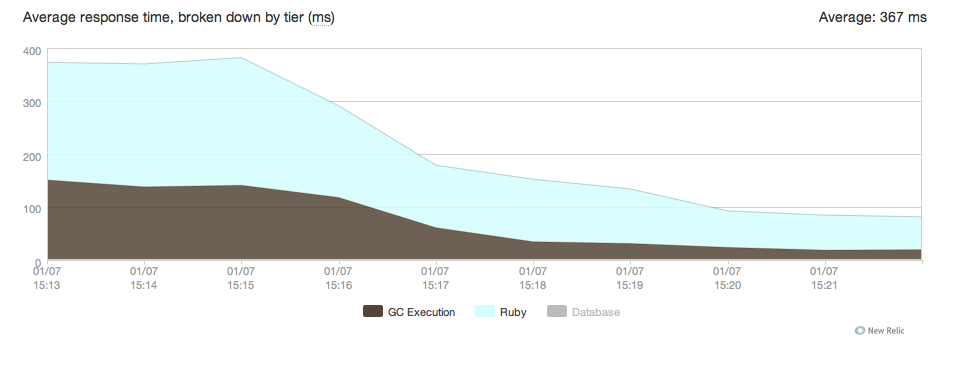
\includegraphics[width=1\textwidth]{figuras/problemas/problemas-stream.png}
  \caption{Tiempo de respuesta promedio después de la migración.\cite{diasp_backbone}}
    \label{fig.problemas-stream}
\end{figure}


\subsubsection{Implementación}

Esta funcionalidad permite agrupar a los contactos de una persona en grupos denominados \emph{aspects}. En particular, cuando un usuario selecciona uno o varios \emph{aspects}
los posts de los mismos aparecen en el stream. El principal inconveniente que se enfrentó durante la migración es que la funcionalidad en sí no estaba funcionando de forma
esperada. No permitía seleccionar más de un \emph{aspect} a la vez, ni recordaba los \emph{aspects} seleccionados y los links de \emph{Select All} y \emph{Deselect All} no
funcionaban.

Esto implicó investigar todos los problemas reportados en \href{https://github.com/diaspora/diaspora/issues?state=open} relacionados a esta funcionalidad para poder determinar bien
cómo era el comportamiento esperado y discutir con los responsables del repositorio en el \emph{irc} del mismo. Una vez resuelta la especificación de la funcionalidad, comenzó el
proceso de diseño de los modelos, colecciones y vistas en \emph{Backbone}, además de los correspondientes \emph{templates} en \emph{Handlebars}. Por otro lado, hubo que eliminar todas
las vistas, código Javascript y acciones en los controladores relacionadas con esta funcionalidad.

\subsubsection{Modelos}

Se creó el modelo \emph{Aspect} en \emph{Backbone} bajo el directorio\\
\emph{app/assets/javascripts/app/models/}. El mismo representa un \emph{aspect} en el listado de los mismos.
Mantiene su estado, en particular si se encuentra seleccionado o no, y provee un método \emph{toggleSelected} para cambiar su estado.

Por otro lado también se agregó el modelo \emph{StreamAspects} el cual hereda de \emph{Stream} y contiene la colección de posts de los \emph{aspects} que se encuentran
seleccionados.

\subsubsection{Colecciones}

Se creó la colección \emph{Aspects} en \emph{Backbone} bajo el directorio\\ 
\emph{app/assets/javascripts/app/collections/}, especificándole el tipo de modelo que la misma va a contener. La
misma mantiene el conjunto de \emph{aspects} del usuario actual y  provee cinco métodos:

\begin{itemize}
\item{selectedAspects(attribute):}

Retorna una lista que contiene el valor del atributo pasado como parámetro de todos los \emph{aspects} de la colección que se encuentran seleccionados.
\item{allSelected:}

Retorna true en caso que todos los \emph{aspects} de la colección estén seleccionados.
\item{selectAll:}

Cambia el valor del atributo \emph{selected} a verdadero de cada elemento de la colección.
\item{deselectAll:}

Cambia el valor del atributo \emph{selected} a falso de cada elemento de la colección.
\item{toSentence:}

Retorna un \emph{string} con los nombres de los \emph{aspects} que se encuentran seleccionados separados por comas, siendo el último separado por la conjunción \emph{y}. En
caso de que no se encuentren \emph{aspects} seleccionados, retorna el \emph{string} \emph{My Aspects}. Tanto los separadores utilizados como el \emph{string} \emph{aspects}
pueden ser traducidos mediante el uso de archivos de configuración y el módulo Diaspora.I18n.
\end{itemize}

\subsubsection{Vistas}

Se crearon dos vistas de \emph{Backbone}: \emph{AspectsList} y \emph{Aspect}. Los \emph{templates} de \emph{Handlebars} correspondientes son \emph{aspects-list} y
\emph{aspect} respectivamente. \emph{AspectsList} es responsable de \emph{renderizar} cada \emph{aspect} de la colección que tiene asociada, para los cuales, crea una vista del
tipo \emph{Aspect}, invoca el método \emph{render} sobre la misma e inserta el elemento retornado al DOM mediante el uso de la función \emph{before} de Jquery en la lista de
\emph{aspects} del sitio. 

Por otro lado, esta vista responde al evento \emph{change} de la colección, el mismo es disparado cuando el estado de alguno de sus elementos cambia. En la inicialización de la
misma se crea un \emph{binding} entre este evento y las funciones \emph{toggleSelector} y \emph{updateStreamTitle}. La primera se encarga de actualizar el texto del link
\emph{Select All} o \emph{Deselect All} en caso de que todos o ninguno de los \emph{aspects} de la colección se encuentren seleccionados. La segunda es responsable de actualizar
el título del \emph{stream} en base a los \emph{aspects} que se encuentran seleccionados. 

Esta vista también responde al evento \emph{click} de Jquery sobre el selector ``.toggle\_selector'' que corresponde al link \emph{Select All}, el cual tienen \emph{bindeado} la
 ejecución de la función \emph{toggleAll}. La misma se encarga de invocar a las funciones \emph{selectAll} o \emph{deselectAll} sobre la colección que tiene la vista asociada.


En cambio la vista \emph{Aspect} se encarga de toda interacción con un elemento en particular. La misma tiene \emph{binding} entre el evento \emph{click} de JQuery sobre el
selector ``.aspect\_selector'' (selector que tiene cada \emph{aspect} en el DOM) y la función \emph{toggleAspect}. La misma se encarga de modificar el valor del atributo
\emph{selected}  del modelo asociado a la vista, de agregarle o quitarle la clase css \emph{active} y de actualizar el \emph{stream} con los posts de los \emph{aspects} que se
encuentran seleccionados.

\subsubsection{Router}

Se agregaron dos funciones más al router de \emph{Backbone}, siendo las mismas \emph{aspects} y \emph{aspects\_stream} las cuales responden a las urls \emph{/aspects} y
\emph{/aspects/stream} respectivamente. Cada vez que se visita una de estas urls, se ejecutan las funciones correspondientes.

La función \emph{aspects\_stream} se encarga de obtener los \emph{aspects} que se encuentran seleccionados, instanciar un modelo del tipo \emph{StreamAspects} y realizar un pedido al
servidor por los posts correspondientes a esos \emph{aspects}. Instancia una  vista del tipo \emph{Stream} con los \emph{posts} obtenidos e invoca el método \emph{render} sobre la misma,
de forma de desplegar los \emph{posts} en el sitio. Por otro lado, en caso de no existir, instancia el \emph{Publisher} (objeto implementado en Javascript encargado del formulario para
generar posts), instancia una vista del tipo StreamFaces (encargada de mostrar la foto de cada \emph{aspect} que tiene un post en el \emph{stream} en la esquina superior derecha
del sitio) e invoca el método \emph{render} sobre la misma.

La función \emph{aspects} por otro lado, se encarga de crear una colección del tipo \emph{Aspects} con la información que se encuentra en el objeto \emph{currentUser} (el mismo
es creado en el servidor y contiene toda la información relevante del usuario actual). Instancia una vista del tipo \emph{AspectsList}, invoca al método \emph{render} sobre la misma y
por último invoca a  la función \emph{aspects\_stream} para desplegar los posts de los mismos.

\subsubsection{Pruebas}

Para realizar las pruebas unitarias de los modelos y vistas que se agregaron a \emph{Backbone} se utilizó Jasmine. Jasmine un framework BDD para testear código Javascript creado por
Pivotal Labs, el repositorio oficial del mismo es \url{https://github.com/pivotal/jasmine}. Este no depende de otros frameworks de Javascript, no requiere el DOM y provee una
sintaxis clara y obvia, la cual permite escribir pruebas de manera sencilla.

Se realizaron pruebas de manera unitaria cada función definida en los modelos, colecciones y vistas nuevas, de forma de tener el mayor cubrimiento posible del código y de las
funcionalidades. Para las pruebas de integración se utilizó cumber y selenium, en particular se agregaron pruebas para que los bugs que existían no resurjan en el futuro.

\subsubsection{Propuesta de la mejora}

Esta mejora se propuso al repositorio oficial y fue aceptada por los responsables del mismo. Las únicas modificaciones requeridas para que el patch fuera aceptado, fueron que todos
los textos sean traducibles. Este patch formó parte de la versión 0.0.3.0 de \emph{Diaspora}.
